
\chapter{研究 : BdG間及びZeromode-BdG間の相互作用を取り入れた有限温度系の計算}
熱力学ポテンシャルの摂動論については「高田康民 : 多体問題(朝倉書店, 1999)」を参考にしています.
\section{やりたいこと}
Y.Nakamura, T.Kawaguchi, Y.Torii, and Y.Yamanaka, arXiv:1604.05900v1(2016)の4章「Thermodynamical quantity and Partition Function」の式(43)では分配関数を
\begin{eqnarray}
  Z = Z_{\rm u, z}Z_{\rm u,ex}
\end{eqnarray}
として評価をしているが, これを
\begin{eqnarray}
  Z = Z_{\rm u, z}Z_{\rm u,ex}Z_{\rm \rm int}
\end{eqnarray}
として評価したい. $Z_{\rm \rm int}$にはゼロモード $\varphi_{z}$ とBdG $\varphi_{\rm ex}$ のカップリング項や$\varphi_{\rm ex}$の高次が含まれている. $Z_{\rm u, z}$と$Z_{\rm u,ex}$は既に解ける形になっているので, 非摂動部の熱力学ポテンシャルを
\begin{eqnarray}
  \Omega_0 = -\frac{1}{\beta}\ln Z_{\rm u, z}Z_{\rm u,ex}
\end{eqnarray}
として$Z_{\rm \rm int}$の効果を摂動的に取り入れたい.
\subsection{Zeromode-BdG coupling}
Hartree-Fock-Bogoliubov approximationによるGP方程式
\begin{eqnarray}
  [h_0 -\mu + g(\xi^2 + 2\ev{\varphi^\dagger\varphi} + \ev{\varphi\varphi})]\xi = 0
\end{eqnarray}
における量子補正$\ev{\varphi^\dagger\varphi}, \ev{\varphi\varphi}$によって既にZeromode-BdGカップリングは導入されているのではないか?:
\begin{eqnarray}
\nonumber  \ev{\varphi^\dagger\varphi} = \ev{(\varphi_z + \varphi_{ex})^\dagger(\varphi_z + \varphi_{ex})} &=& \ev{(\varphi^\dagger_z\varphi_z + \varphi^\dagger_{ex}\varphi_z  + \varphi^\dagger_z\varphi_{ex} + \varphi^\dagger_{ex}\varphi_{ex})}\\
  &=& \ev{\varphi^\dagger_z\varphi_z} + \ev{\varphi^\dagger_{ex}\varphi_{ex}}
\end{eqnarray}
カップリング項は$\varphi$の一次なので消えてしまい, Zeromode-BdGカップリングは導入できていない.

\begin{comment}
\ul{$Z_{\rm \rm int}$を摂動的に取り込んだ結果, その効果がGP方程式やその他の方程式群にどのよう(何を通して)に取り込}\\
\ul{まれるのか. 量子効果を取り込んだ従来のFormulationだとZeromode-BdG間の相互作用は取り入れることがで}\\
\ul{きていなかったのか?} 
\end{comment}

\section{量子統計力学と摂動計算}
熱力学ポテンシャルを用いた摂動計算のための勉強.
\subsection{熱力学ポテンシャル}
熱力学ポテンシャル(グランドポテンシャル, thermodynamic potential)は
\begin{eqnarray}
  \Omega &=& F - \mu N = E - TS -\mu N\\
  d\Omega &=& SdT - Nd\mu -pdV
\end{eqnarray}
のように定義され, 大分配関数を用いて
\begin{eqnarray}
  \Omega &=& -k_BT\ln Z\\
  Z &=& \exp(-\beta\Omega) = \Tr e^{-\beta H}
\end{eqnarray}
のようにも書ける. この熱力学関数のおかげで
\begin{eqnarray}
  S = -\qty(\frac{\partial\Omega}{\partial T})_{\mu, V}\hspace{0.7cm}N = -\qty(\frac{\partial\Omega}{\partial \mu})_{T, V}\hspace{0.7cm}p = -\qty(\frac{\partial\Omega}{\partial V})_{T, \mu}\hspace{0.7cm}C_v = -T\qty(\frac{\partial^2\Omega}{\partial T^2})_{\mu, V} = T\qty(\frac{\partial S}{\partial T})_{\mu, V}
\end{eqnarray}
などの物理量を計算できる. 大分配関数$Z$を求めよう!という大筋は変わらない.
\subsection{方法論の外観}
熱平衡状態を知るためには熱力学ポテンシャルを計算することがまず第一である.
例えば$H$が
\begin{eqnarray}
  H = \sum_n \omega_n a_n^\dagger a_n
\end{eqnarray}
みたいなFreeであるなら
\begin{eqnarray}
  \Omega = -k_BT\ln(\Tr e^{-\beta H}) = -k_BT\ln(\prod_n\frac{1}{1-e^{-\beta \omega_n}}) = k_BT\sum_n\ln(1-e^{-\beta \omega_n})
\end{eqnarray}
みたいに計算はすぐにできるが, 相互作用が入ってきた場合の計算は容易ではない. いろいろな方法論が存在するが, ここでは場の理論を用いた摂動論を扱う.
\subsection{相互作用描像とS行列}
Heisenberg描像のハミルトニアンを
\begin{eqnarray}
  H_{\rm H} = H_{\rm H, u, z} + H_{\rm H, u, ex} + H_{\rm H, \rm int}
\end{eqnarray}
と分割したとき, $H_{\rm u, z}$と$H_{\rm u, ex}$については固有値方程式
\begin{eqnarray}
  H_{\rm u, ex}\ket{n}_{\rm ex} &=& \omega_n\ket{n}_{\rm ex}\\
  H_{\rm u, z}\ket{\Psi_\nu}_{\rm z} &=& E_\nu\ket{\Psi_\nu}_{\rm z}
\end{eqnarray}
が既に解けているものとする\footnote{非摂動部は時間発展しないように選んでいるので, Heisenberg描像$H_{\rm H}$と相互作用描像$H$は一致する}.
ここで, Schr\"odinger描像とHeisenberg描像・相互作用描像を結ぶユニタリー変換を考える:
\begin{eqnarray}
  A_{\rm H}(t) = e^{iH_St}A_Se^{-iH_St}\hspace{1.0cm} &Heisenberg\ picture\label{picture1}\\
  A(t) = e^{iH_ut}A_Se^{-iH_ut}\hspace{1.0cm} &Interaction\ picture\label{picture2}
\end{eqnarray}
$H_u = H_{\rm u, z} + H_{\rm u, ex}$としている.\\
%\ul{(\ref{picture1})のユニタリー変換を司る$H$の描像はナンだ?$H_{\rm S}$と$H_{\rm H}$は同一視していいのか?}
s
これを用いてHeisenberg描像と相互作用描像を結ぶユニタリー変換$U(t)$を定義する:
\begin{eqnarray}
  A_{\rm H}(t) &=& U^{-1}(t)A(t)U(t)\\
  e^{iH_St}A_Se^{-iH_St} &=& U^{-1}(t)e^{iH_ut}A_Se^{-iH_ut}U(t)\\
  \therefore U(t) &=& e^{iH_ut}e^{-iH_St}
\end{eqnarray}
このユニタリー演算子の時間発展方程式は
\begin{eqnarray}
\nonumber  \partial_tU(t) &=& e^{iH_ut}(iH_u)e^{-iH_St} -e^{iH_ut}(-iH_S)e^{-iH_St}\\
  &=& ie^{iH_ut}(H_u - H_S)e^{-iHt} = -ie^{iH_ut}H_{\rm S, ex}e^{-iH_ut}U(t)\\
\therefore i\partial_tU(t) &=& H_{\rm ex}(t)U(t)\label{unitary1}\\
\therefore i\partial_tU^{-1}(t) &=& -U^{-1}(t)H_{\rm ex}(t)\label{unitary2}
\end{eqnarray}
ここでは$H_u = H_{S, u}$を用いている. この$U(t)$を用いて新しい演算子$S(t, t')$を定義する:
\begin{eqnarray}
  S(t, t') = U(t)U^{-1}(t')
\end{eqnarray}
このS行列の時間発展方程式は(\ref{unitary1})より直ちに
\begin{eqnarray}
  i\partial_tS(t, t') &=& H_{\rm ex}(t)S(t, t')
\end{eqnarray}
を得る. これを形式的に解くとT積を用いて
\begin{eqnarray}
  S(t, t') = T\exp[-i\int_{t'}^{t}ds H_{\rm ex}(s)]
\end{eqnarray}
と表現できる.
\subsection{熱力学ポテンシャルの摂動展開}
前節の議論を$it \rightarrow \beta$とする:
\begin{eqnarray}
  U(\beta) &=& e^{\beta H_u}e^{-\beta H_S}\hspace{1cm}\partial_\beta U(\beta) = -H_{\rm ex}(\beta)U(\beta)\\
  S(\beta, \beta') &=& U(\beta)U^{-1}(\beta')\hspace{1cm}\partial_\beta S(\beta, \beta') = -H_{\rm ex}(\beta)S(\beta, \beta')\\
  S(\beta, \beta') &=& T\exp[-\int_{\beta'}^{\beta}ds H_{\rm ex}(s)]
\end{eqnarray}
このS行列を用いて大分配関数$Z$を書き換える:
\begin{eqnarray}
  Z = e^{-\beta\Omega} = \Tr e^{-\beta H} = \Tr[e^{-\beta H_u}U(\beta)]= \Tr[e^{-\beta H_u}S(\beta, 0)]\label{partition}
\end{eqnarray}
ここで, 任意の演算子対して非摂動系における熱平均を定義する. ここでいう任意の演算子は「ゼロモード演算子と励起モード演算子を含む演算子」を指すので, 任意の演算子は$\varphi_{z}\varphi_{ex}$とする:
\begin{eqnarray}
\nonumber  \ev{\varphi_{z}\varphi_{ex}}_0 &=& \frac{\Tr\qty[e^{-\beta H_u}\varphi_{z}\varphi_{ex}]}{\Tr\qty[e^{-\beta H_u}]} = e^{\beta\Omega_0}\sum_{mn}\ _z\!\bra{\Psi_m}\otimes\ _{ex}\!\bra{n}e^{-\beta H_u}\varphi_z\varphi_{ex} \ket{\Psi_m}_z\otimes\ \ket{n}_{ex}\\
\nonumber  &=& e^{\beta\Omega_0}\sum_{mn}\ _z\!\bra{\Psi_m}e^{-\beta H_z}\varphi_z\ket{\Psi_m}_z\otimes\ _{ex}\!\bra{n}e^{-\beta H_{ex}}\varphi_{ex}\ket{n}_{ex}\\
  &=& e^{\beta\Omega_0}\Tr_{z}\qty[e^{-\beta H_z}\varphi_z]\Tr_{ex}\qty[e^{-\beta H_{ex}}\varphi_{ex}] = \ev{\varphi_z}_z\ev{\varphi_{ex}}_{ex}
\end{eqnarray}
$\Omega_0 = -\beta^{-1}\ln Z_0$であり, $\Tr_z, \Tr_{ex}$はそれぞれ, ゼロモード部・励起部をトレースアウトする操作を表している. この定義より, 大分配関数(\ref{partition})は





\begin{comment}
\begin{eqnarray}
  \nonumber Z &=& \Tr[e^{-\beta H_u}S(\beta, 0)] = e^{-\beta\Omega_0}\ev{S(\beta, 0)_z}_z\ev{S(\beta, 0)_{ex}}_{ex}\\
  &=& e^{-\beta\Omega_0}\ev{T\exp\qty[-\int_0^\beta dsH_{Iz}(s)]}_z\ev{T\exp\qty[-\int_0^\beta dsH_{Iex}(s)]}_{ex}\label{Perturbed-thermo1}
\end{eqnarray}
$S(\beta, 0)_z, S(\beta, 0)_{ex}, H_{Iz}, H_{Iz}$はそれぞれ, $S(\beta, 0), H_{ex, z}$をゼロモード部と励起部に分けたものと便宜的に置いている. \textbf{$S(\beta, 0)$をゼロモード部と励起部に単純に分割できるかどうかはまだ一切議論していないことに注意. } 以上のことを仮定すると熱力学ポテンシャル$\Omega$は
\begin{eqnarray}
\nonumber  \Omega &=& -\frac{1}{\beta}\ln Z = -\frac{1}{\beta}\ln\qty(e^{-\beta\Omega_0}\ev{T\exp\qty[-\int_0^\beta dsH_{Iz}(s)]}_z\ev{T\exp\qty[-\int_0^\beta dsH_{Iex}(s)]}_{ex})\\
  &=& \Omega_0 - \frac{1}{\beta}\ln\ev{T\exp\qty[-\int_0^\beta dsH_{Iz}(s)]}_z- \frac{1}{\beta}\ln\ev{T\exp\qty[-\int_0^\beta dsH_{Iex}(s)]}_{ex}\label{Perturbed-thermo2}
\end{eqnarray}
熱力学ポテンシャルを求めるためには, (\ref{Perturbed-thermo2})の右辺第2・3項の摂動的評価が必要がある.
\end{comment}

\begin{eqnarray}
  Z &=& \Tr[e^{-\beta H_u}S(\beta, 0)] = e^{-\beta\Omega_0}\ev{T\exp[-\int_0^\beta ds H_{\rm int}(s)]}_0\\
  \therefore \Omega &=& \Omega_0 -\frac{1}{\beta}\ln\ev{T\exp[-\int_0^\beta ds H_{\rm int}(s)]}_0\label{Perturbed-thermo2}
\end{eqnarray}
この$\ev{\bullet}_0$が$\ev{\bullet}_{z}\ev{\bullet}_{ex}$に分解できるかどうかが後々議論する. 

\subsection{描像について}
描像について少々雑に議論していたのではないだろうか?ゼロモード部と励起部の時間依存性についてもう少し詳細に見ていくことにする. $H_{S, ex, z} = \varphi_{S, z}\varphi_{S, ex}$として相互作用描像$H_{ex, z}(t)$を
\begin{eqnarray}
  H_{ex, z}(t) = e^{iH_ut}H_{S, ex, z}e^{-iH_ut} = e^{iH_{u, z}t}e^{iH_{u, ex}t}\varphi_{S, z}\varphi_{S, ex}e^{-iH_{u, z}t}e^{-iH_{u, ex}t}
\end{eqnarray}
$\varphi_{ex}$と$H_{u, ex}$は$H_{u, z}$と交換し, 同様に$\varphi_{z}$と$H_{u, z}$は$H_{u, ex}$と交換することから
\begin{eqnarray}
  H_{ex, z}(t) = e^{iH_{u, z}t}\varphi_{S, z}e^{-iH_{u, z}t}e^{iH_{u, ex}t}\varphi_{S, ex}e^{-iH_{u, ex}t} = \varphi_{z}(t)\varphi_{ex}(t)
\end{eqnarray}
となる. (\ref{picture2})は正しそう. 故にHeisenberg描像と相互作用描像を結ぶユニタリー変換$U(t)$やS行列$S(t, t')$, それら時間発展は修正を受けない.
\section{3次元有限温度IZMF系への応用}
\subsection{ハミルトニアン}
3次元調和トラップ系で考える. 秩序変数$\xi$と共役モード$\eta$が実であるような流れのない凝縮体を仮定する. また$\xi, \eta$が時間依存しないことを要請する. 以下, 各記号は元論文の表式に従う. 

相互作用描像におけるハミルトニアンを
\begin{eqnarray}
  H = H_1 + H_2 + H_3 + H_4
\end{eqnarray}
と分割.$\varphi$の次数ごとに
\begin{eqnarray}
  H_1 &=& \int d\bm{x} \left[ \varphi^\dagger(h_0 -\mu + g|\xi|^2)\xi + \varphi(h_0 - \mu + g|\xi|^2)\xi^* \right]\\
  H_2 &=& \frac{1}{2}\int d\bm{x}
  \begin{pmatrix}
    \varphi^\dagger & -\varphi
  \end{pmatrix}
  T_0
  \begin{pmatrix}
    \varphi\\
    \varphi^\dagger
  \end{pmatrix}
  \\
  H_3 &=& g\int g\bm{x} \left[ \varphi^\dagger\varphi^\dagger\varphi\xi + \varphi^\dagger\varphi\varphi\xi^* \right]\\
  H_4 &=& \frac{g}{2}\int d\bm{x} \varphi^\dagger\varphi^\dagger\varphi\varphi
\end{eqnarray}
としている.場の演算子を$\varphi = \varphi_{z} + \varphi_{ex}$のように分割. それぞれ以下のようになる:
\begin{eqnarray}
  \varphi_{z} &=& -i\xi Q + \eta P\label{Zeromode-expansion}\\
  \varphi_{ex} &=& \sum_j \qty[u_ja_j + v_j^*a_j^\dagger]\label{plane}
\end{eqnarray}
BdG方程式の正ノルムの固有関数を$y_j = (u_j, v_j)^t$としている. 非摂動ハミルトニアンのゼロモード部・励起部は
\begin{eqnarray}
  \nonumber H_{u, z} &=& -(\delta\mu +4C)P + \frac{I - 4D}{2}P^2 + 2BQPQ + 2DP^3\\
  &&\hspace{3.5cm} +\frac{1}{2}AQ^4- 2BQ^2 + CQP^2Q + \frac{1}{2}EP^4\\
  H_{u, ex} &=& \int d\bm{x} \qty[\varphi^\dagger_{ex}{\cal L}\varphi_{ex} + \frac{1}{2}\varphi_{ex}{\cal M}^*\varphi_{ex} + \frac{1}{2}\varphi^\dagger_{ex}{\cal M}\varphi^\dagger_{ex}]
\end{eqnarray}
とする. 摂動項は
\begin{eqnarray}
    \nonumber  H_{\rm int} &=& g\int d\bm{x} \Bigl[\varphi_z^\dagger\calL\varphi_{ex} + \varphi_{ex}^\dagger\calL\varphi_z + \varphi_z\calM^*\varphi_{ex} + \varphi_z^\dagger\calM\varphi_{ex}^\dagger\\
    \nonumber  && +\ \xi^*(2\varphi_z^\dagger\varphi_z\varphi_{ex} + \varphi_z^\dagger\varphi_{ex}\varphi_{ex} + 2\varphi_{ex}^\dagger\varphi_z\varphi_{ex} + \varphi_{ex}^\dagger\varphi_z\varphi_z)\\
    \nonumber  && +\ \xi\ (2\varphi_z^\dagger\varphi_{ex}^\dagger\varphi_z + \varphi_z^\dagger\varphi_z^\dagger\varphi_{ex} + 2\varphi_z^\dagger\varphi_{ex}^\dagger\varphi_{ex} + \varphi_{ex}^\dagger\varphi_{ex}^\dagger\varphi_z)\\
  \nonumber  && +\ 2(\varphi^\dagger_z\varphi^\dagger_z\varphi_z\varphi_{ex} + \varphi^\dagger_z\varphi^\dagger_{ex}\varphi_z\varphi_z + \varphi_{ex}^\dagger\varphi^\dagger_{ex}\varphi_{ex}\varphi_{z} + \varphi^\dagger_{ex}\varphi^\dagger_{z}\varphi_{ex}\varphi_{ex}) \\
    && +\ \varphi^\dagger_z \varphi^\dagger_z \varphi_{ex}\varphi_{ex} + 4\varphi^\dagger_z \varphi_z \varphi^\dagger_{ex}\varphi_{ex} + \varphi_z \varphi_z \varphi^\dagger_{ex}\varphi^\dagger_{ex} + \varphi_{ex}^\dagger\varphi_{ex}^\dagger\varphi_{ex}\varphi_{ex}\Bigr]\label{ZeromodeHamiltonian}
\end{eqnarray}
のように, そこそこ煩雑です. ただし, 摂動展開の線形部分だけを見るのであれば$\varphi_{ex}, \varphi_z$の奇数次は落ちてくれるのでもう少し簡単になるでしょう. もちろん2次まで見るとなるとかなりキツくなると思われます.
\subsection{熱力学ポテンシャルの具体形}
(\ref{Perturbed-thermo2})の1次について具体形を書き下す. 
\begin{eqnarray}
\nonumber  T\exp[-\int_0^\beta ds H_{\rm int}(s)] &=& I -\int_0^{\beta}ds H_{\rm int}(s) + \frac{1}{2!}\int_0^\beta ds\int_0^\beta ds' T\qty[H_{\rm int}(s)H_{\rm int}(s')] + \cdots\\
 \therefore \ev{T\exp[-\int_0^\beta ds H_{\rm int}(s)]}_0 &\simeq& \ev{I -\int_0^{\beta}ds H_{\rm int}(s)}_0 =  1 - \int_0^\beta ds\ev{H_{\rm int}(s)}_0\label{Perturbed-thermo3}
%&=& 1 - e^{\beta\Omega_0}\sum_{mn}\int_0^\beta ds\bra{\Psi_m}\bra{n}e^{-\beta H_u}H_{\rm int}(s)\ket{n}\ket{\Psi_m}
\end{eqnarray}
ここで(\ref{Perturbed-thermo3})の積分内の期待値はゼロモード項と励起項に分離でき, 期待値が残るのは$\varphi_z, \varphi_{ex}$の2次及び$\varphi_{ex}$の4次のみである. 書き下すと
\begin{eqnarray}
  \nonumber  \ev{H_{\rm int}}_0 &=& \int d\bx\Bigl[\ev{\varphi_z^\dagger(s)\varphi_z^\dagger(s)}_z\ev{\varphi_{ex}(s)\varphi_{ex}(s)}_{ex} + 4\ev{\varphi_z^\dagger(s)\varphi_z(s)}_z\ev{\varphi_{ex}^\dagger(s)\varphi_{ex}(s)}_{ex}\\
  &+& \ev{\varphi_z(s)\varphi_z(s)}_z\ev{\varphi_{ex}^\dagger(s)\varphi_{ex}^\dagger(s)}_{ex} + \ev{\varphi_{ex}^\dagger(s)\varphi_{ex}^\dagger(s)\varphi_{ex}(s)\varphi_{ex}(s)}_{ex}\Bigr]\label{Hamiltonian-Exp}
\end{eqnarray}
% ---------- Comment out -------------
\begin{comment}
\begin{eqnarray}
  \nonumber  &&\bra{\Psi_m}\bra{n}e^{-\beta H_u}H_{\rm int}(s)\ket{n}\ket{\Psi_m}\\
\nonumber  &=& e^{-\beta(E_m + \omega_n)}\Bigl[\ev{\varphi^\dagger_z(s)\varphi^\dagger_z(s)}{\Psi_m}\ev{\varphi_{ex}(s)\varphi_{ex}(s)}{n} + 4\ev{\varphi^\dagger_z(s)\varphi_z(s)}{\Psi_m}\ev{\varphi^\dagger_{ex}(s)\varphi_{ex}(s)}{n}\\
\nonumber  &&\hspace{2cm} + \ev{\varphi_z(s)\varphi_z(s)}{\Psi_m}\ev{\varphi^\dagger_{ex}(s)\varphi^\dagger_{ex}(s)}{n}\Bigr] + e^{-\beta\omega_n}\ev{\varphi^\dagger_{ex}(s)\varphi^\dagger_{ex}(s)\varphi_{ex}(s)\varphi_{ex}(s)}{n}\\
\end{eqnarray}
\end{comment}
% ---------- Comment out -------------
(\ref{Zeromode-expansion})(\ref{plane})の展開を用いると, 効いてくるのは
\begin{eqnarray}
  &&\ev{Q^2(s)}_z\hspace{0.7cm}\ev{P^2(s)}_z\hspace{0.7cm}\ev{a_{\bk}^\dagger(s) a_{\bk'}(s)}_{ex}\hspace{0.7cm}\ev{a_{\bk_1}^\dagger(s)a_{\bk_2}^\dagger(s) a_{\bk_3}(s)a_{\bk_4}(s)}_{ex}
\end{eqnarray}
のような項たち. 具体形は
\begin{eqnarray}
  \ev{Q^2(s)}_z &=& \frac{\sum_m\int dqq^2|\Psi_m(q)|^2e^{-\beta E_m}}{\sum_me^{-\beta E_m}}\\
  \ev{P^2(s)}_z &=& \frac{-\sum_m\frac{d^2}{dq^2}|\Psi_m(q)|^2e^{-\beta E_m}}{\sum_me^{-\beta E_m}}\\
  \ev{a_{\bk}^\dagger(s) a_{\bk'}(s)}_{ex} &=& \frac{1}{e^{\beta\omega_{\bk}}-1}\delta_{\bk, \bk'} \equiv n_{\bk}\delta_{\bk, \bk'}\\
\nonumber  \ev{a_{\bk_1}^\dagger(s)a_{\bk_2}^\dagger(s) a_{\bk_3}(s)a_{\bk_4}(s)}_{ex} &=& \qty(\wick{12}{<1a^\dagger_{k1}<2a^\dagger_{k2}>1a_{k3}>2a_{k4}} + \wick{12}{<1a^\dagger_{k1}<2a^\dagger_{k2}>2a_{k3}>1a_{k4}})\\
  &=& n_{\bk_1}n_{\bk_2}\qty(\delta_{\bk_1, \bk_3}\delta_{\bk_2, \bk_4} + \delta_{\bk_1, \bk_4}\delta_{\bk_2, \bk_3}) = 2n_{\bk_1}n_{\bk_2}
\end{eqnarray}
である. ゼロモード期待値は$q$-表示を採用している\footnote{$q$表示というのは実空間の$q$ではなく, いわゆるゼロモード空間の$q$表示. もちろん空間のサイズは実空間に依存せず, 数値計算の際には適切なサイズを用意しなければならない. }. $\Psi_m$は非摂動ゼロモードハミルトニアン$H_{u, z}$の固有状態.

\subsection{$a(s)$の時間依存性}
相互作用描像なので演算子の時間依存性についての議論が必要. 非摂動ハミルトニアンが
\begin{eqnarray}
  H_{u, ex} = \int d\bk\ \omega_k a^\dagger(t) a(t)
\end{eqnarray}
のように対角化されていれば, 時間成分は
\begin{eqnarray}
  i\partial_ta(t) &=& [a(t), H_u] = \omega_k a(t)\\
 \therefore a(t) &=& a(0)e^{-i\omega_k t}
\end{eqnarray}
のようにくくり出せる. よって, $a^\dagger(t) a(t), a^\dagger(t) a^\dagger(t) a(t)a(t)$の時間依存性は消える. 
\subsection{$Q(s), P(s)$の時間依存性}
あるゼロモード演算子$A(t)$の期待値の時間発展は
\begin{eqnarray}
  i\partial_t \bra{\Psi} A(t) \ket{\Psi}
  = \bra{\Psi} A(t) H_u - H_u A(t) \ket{\Psi}
= \bra{\Psi} A(t) E_n - E_n A(t) \ket{\Psi}
= 0
\end{eqnarray}
のようにゼロになることがわかる. ゼロモードの真空はもちろん時間発展しない. 励起
部は時間発展するものの, それは位相の回転にあたる.  ブラとケットで逆向きに回るた
め期待値には効いてこない. ということで, ゼロモード期待値も時間依存性を持たない. 

\subsection{$Q, P$を奇数個含むエルミートな期待値がゼロになること}
$\xi, \eta$が実の場合で, かつ今回選んだゼロモードハミルトニアンは$Q$の奇数次が存在しないので, $p$表示したゼロモードハミルトニアンは実対称行列になっている. よって, $p$表示のゼロモード方程式
\begin{eqnarray}
  H_{u, z}(p)\bra{p}\ket{\Psi} = E_0\bra{p}\ket{\Psi}
\end{eqnarray}
において, $\bra{p}\ket{\Psi}$を実の固有ベクトルとして選ぶことができる. $\bra{p}\ket{\Psi}$が実であるならば
\begin{eqnarray}
\nonumber  \bra{\Psi}Q^3\ket{\Psi} &=& \int dp \bra{\Psi}Q^3\ket{p}\bra{p}\ket{\Psi} = \int dp \Psi(p)\qty(i\frac{d}{dp})^3\Psi(p)= -\int dp \qty(i\frac{d}{dp})^3\Psi(p)\Psi(p)\\
\therefore &&\int dp \Psi(p)\qty(i\frac{d}{dp})^3\Psi(p) + \int dp \qty(i\frac{d}{dp})^3\Psi(p)\Psi(p) = 2\bra{\Psi}Q^3\ket{\Psi} = 0
\end{eqnarray}
のように, $Q$の奇数次の期待値はゼロになる. 一行目では部分積分を用いている. 同様に, $QP + PQ$などの$Q$の奇数次を含むエルミートな期待値もゼロになるが, $QP$はエルミートでないのでその限りではない. 

Full Hamiltonianに含まれる全てのゼロモード演算子を取り入れたようなゼロモードハミルトニアンには$Q$の奇数次は存在しないが, $P$の奇数次は存在する. しかしながら, 今回選んだ$H_{u, z}$には$P$の奇数次も存在しない\footnote{物理量に対するゼロモードの奇数次の寄与が小さいだろうという仮定のもと.\ul{これが今回適当かどうかはよくわかりません.} }ので, 同様の議論から$P$の奇数次及び, $P$の奇数次を含むエルミートな期待値もゼロになることがわかる.

\subsection{(\ref{Hamiltonian-Exp})のさらなる具体形}
時間依存性を考慮しなくて良いことがわかったのでさらに議論をすすめて数値計算が可能な形まで落としこむことにする. まず, (\ref{Hamiltonian-Exp})のゼロモード部について. 先ほど同様, $Q$のエルミートな奇数次項を落とすと
\begin{eqnarray}
\nonumber  \ev{\varphi^\dagger_z\varphi^\dagger_z}_z &=& \ev{(-i\xi Q + \eta P)^\dagger(-i\xi Q + \eta P)^\dagger}_z = -\xi^2\ev{Q^2}_z + \eta^2\ev{P^2}_z\\
\nonumber \ev{\varphi_z^\dagger\varphi_z}_z &=& \xi^2\ev{Q^2}_z + \eta^2\ev{P^2}_z - i\xi\eta\\
\ev{\varphi_z\varphi_z}_z &=& -\xi^2\ev{Q^2}_z + \eta^2\ev{P^2}_z\label{Zeromode-Exp}
\end{eqnarray}
一方で励起部は
\begin{eqnarray}
  \ev{\varphi_{ex}\varphi_{ex}}_{ex} &=& \sum_j\qty[2*n_j + 1]u_jv_j^*\label{BdG-Exp}\\
  \ev{\varphi_{ex}^\dagger\varphi_{ex}}_{ex} &=& \sum_j\qty[n_j(|u_j|^2 + |v_j|^2) + |v_j|^2]
\end{eqnarray}
相互作用項は
\begin{eqnarray}
\nonumber \ev{\varphi_{ex}^\dagger\varphi_{ex}^\dagger\varphi_{ex}\varphi_{ex}}_{ex} &=& \sum_{\bk1, \bk2, \bk3, \bk4}\qty(u_{\bk_1}a_{\bk_1} + v_{\bk_1}^*a_{\bk_1}^\dagger)^\dagger\qty(u_{\bk_2}a_{\bk_2} + v_{\bk_2}^*a_{\bk_2}^\dagger)^\dagger\qty(u_{\bk_3}a_{\bk_3} + v_{\bk_3}^*a_{\bk_3}^\dagger)\qty(u_{\bk_4}a_{\bk_4} + v_{\bk_4}^*a_{\bk_4}^\dagger)\\
\end{eqnarray}
である. 生成演算子と消滅演算子が対になっていない期待値は消えてしまうので, 残るものだけを書き下す:
\begin{eqnarray}
  \nonumber\ev{\varphi_{ex}^\dagger\varphi_{ex}^\dagger\varphi_{ex}\varphi_{ex}}_{ex} &=& \sum_{\bk1, \bk2, \bk3, \bk4}
  \Bigl[u_{\bk_1}^*u_{\bk_2}^*u_{\bk_3}u_{\bk_4}\ev{a^\dagger_{\bk_1}a^\dagger_{\bk_2}a_{\bk_3}a_{\bk_4}}_{ex} + u_{\bk_1}^*v_{\bk_2}u_{\bk_3}v_{\bk_4}^*\ev{a^\dagger_{\bk_1}a_{\bk_2}a_{\bk_3}a^\dagger_{\bk_4}}_{ex}\\
    \nonumber    &&+ u_{\bk_1}^*v_{\bk_2}v_{\bk_3}^*u_{\bk_4}\ev{a^\dagger_{\bk_1}a_{\bk_2}a^\dagger_{\bk_3}a_{\bk_4}}_{ex} + v_{\bk_1}u_{\bk_2}^*u_{\bk_3}v_{\bk_4}^*\ev{a_{\bk_1}a^\dagger_{\bk_2}a_{\bk_3}a^\dagger_{\bk_4}}_{ex}\\
\nonumber    &&+ v_{\bk_1}u_{\bk_2}^*v_{\bk_3}^*u_{\bk_4}\ev{a_{\bk_1}a^\dagger_{\bk_2}a^\dagger_{\bk_3}a_{\bk_4}}_{ex} + v_{\bk_1}v_{\bk_2}v_{\bk_3}^*v_{\bk_4}^*\ev{a_{\bk_1}a_{\bk_2}a^\dagger_{\bk_3}a^\dagger_{\bk_4}}_{ex}\Bigr]\\\label{interactionexpectation}
\end{eqnarray}
Wickの定理で展開:
\begin{eqnarray}
\nonumber  \ev{a^\dagger_{\bk_1}a^\dagger_{\bk_2}a_{\bk_3}a_{\bk_4}}_{ex} &=& \qty(\wick{12}{<1a^\dagger_{k1}<2a^\dagger_{k2}>1a_{k3}>2a_{k4}} + \wick{21}{<1a^\dagger_{k1}<2a^\dagger_{k2}>2a_{k3}>1a_{k4}})\\
&=& n_{\bk_1}n_{\bk_2}\qty(\delta_{\bk_1, \bk_3}\delta_{\bk_2, \bk_4} + \delta_{\bk_1, \bk_4}\delta_{\bk_2, \bk_3})\\
\nonumber  \ev{a^\dagger_{\bk_1}a_{\bk_2}a_{\bk_3}a^\dagger_{\bk_4}}_{ex} &=& \qty(\wick{12}{<1a^\dagger_{k1}>1a_{k2}<2a_{k3}>2a^\dagger_{k4}} + \wick{12}{<1a^\dagger_{k1}<2a_{k2}>1a_{k3}>2a^\dagger_{k4}})\\
\nonumber&=& n_{\bk_1}(1 + n_{\bk_3})\delta_{\bk_1, \bk_2}\delta_{\bk_3, \bk_4} + n_{\bk_1}(1 + n_{\bk_2})\delta_{\bk_1, \bk_3}\delta_{\bk_2, \bk_4}\\
\\
\nonumber  \ev{a^\dagger_{\bk_1}a_{\bk_2}a^\dagger_{\bk_3}a_{\bk_4}}_{ex} &=& \qty(\wick{12}{ <1a^\dagger_{k_1}>1a_{k_2}<2a^\dagger_{k_3}>2a_{k_4}} + \wick{21}{<1a^\dagger_{k_1}<2a_{k_2}>2a^\dagger_{k_3}>1a_{k_4}})\\
&=& n_{\bk_1}n_{\bk_3}\delta_{\bk_1, \bk_2}\delta_{\bk_3, \bk_4} + n_{\bk_1}(1 + n_{\bk_2})\delta_{\bk_1, \bk_4}\delta_{\bk_2, \bk_3}\\
\nonumber  \ev{a_{\bk_1}a^\dagger_{\bk_2}a_{\bk_3}a^\dagger_{\bk_4}}_{ex} &=& \qty(\wick{12}{<1a_{k_1}>1a^\dagger_{k_2}<2a_{k_3}>2a^\dagger_{k_4}} + \wick{21}{<1a_{k_1}<2a^\dagger_{k_2}>2a_{k_3}>1a^\dagger_{k_4}})\\
\nonumber&=& (1+n_{\bk_1})(1+n_{\bk_3})\delta_{\bk_1, \bk_2}\delta_{\bk_3, \bk_4} + (1+n_{\bk_1})n_{\bk_2}\delta_{\bk_1, \bk_4}\delta_{\bk_2, \bk_3}\\
\\
\nonumber  \ev{a_{\bk_1}a^\dagger_{\bk_2}a^\dagger_{\bk_3}a_{\bk_4}}_{ex} &=& \qty(\wick{12}{<1a_{k_1}>1a^\dagger_{k_2}<2a^\dagger_{k_3}>2a_{k_4}} + \wick{12}{<1a_{k_1}<2a^\dagger_{k_2}>1a^\dagger_{k_3}>2a_{k_4}})\\
&=& (1 + n_{\bk_1})n_{\bk_3}\delta_{\bk_1, \bk_2}\delta_{\bk_3, \bk_4} + (1 + n_{\bk_1})n_{\bk_2}\delta_{\bk_1, \bk_3}\delta_{\bk_2, \bk_4}\\
\nonumber  \ev{a_{\bk_1}a_{\bk_2}a^\dagger_{\bk_3}a^\dagger_{\bk_4}}_{ex} &=& \qty(\wick{12}{<1a_{k_1}<2a_{k_2}>1a^\dagger_{k_3}>2a^\dagger_{k_4}} + \wick{21}{<1a_{k_1}<2a_{k_2}>2a^\dagger_{k_3}>1a^\dagger_{k_4}})\\
&=& (1 + n_{\bk_1})(1 + n_{\bk_2})\qty(\delta_{\bk_1, \bk_3}\delta_{\bk_2, \bk_4} + \delta_{\bk_1, \bk_4}\delta_{\bk_2, \bk_3})
\end{eqnarray}
これらを(\ref{interaction-expectation})に代入すると
\begin{eqnarray}
  \nonumber \ev{\varphi_{ex}^\dagger\varphi_{ex}^\dagger\varphi_{ex}\varphi_{ex}}_{ex} &=& \sum_{j_1, j_2}\Bigl[\qty(2|u_{j_1}|^2|u_{j_2}|^2 + u_{j_1}^*v_{j_1}v_{j_2}^*u_{j_2})n_{j_1}n_{j_2}\\
\nonumber  &+& \qty(2\Re\qty[u_{j_1}^*v_{j_1}u_{j_2}v_{j_2}^*] + 4|u_{j_1}|^2|v_{j_2}|^2)n_{j_1}(1+n_{j_2})\\ &+& \qty(2|v_{j_1}|^2|v_{j_2}|^2 + v_{j_1}u_{j_1}^*u_{j_2}v_{j_2}^*)(1+n_{j_1})(1+n_{j_2})\Bigr]\label{Interaction-Exp}
\end{eqnarray}
となる. 

以上で具体的にゼロモード・励起モードの期待値が計算できたので, (\ref{Hamiltonian-Exp})に(\ref{Zeromode-Exp}), (\ref{BdG-Exp}), (\ref{Interaction-Exp})を代入する. まとめると, (\ref{Hamiltonian-Exp})は
\begin{eqnarray}
  \nonumber  \ev{H_{\rm int}}_0 &=& \int d\bx\sum_j\Bigl[2\qty(-\xi^2\ev{Q^2}_z + \eta^2\ev{P^2}_z)\qty(2n_j + 1)u_jv_j^*\\
    &+& 4\qty(\xi^2\ev{Q^2}_z + \eta^2\ev{P^2}_z - \xi\eta)\qty[n_j(|u_j|^2 + |v_j|^2) + |v_j|^2] + \ev{\varphi_{ex}^\dagger\varphi_{ex}^\dagger\varphi_{ex}\varphi_{ex}}_{ex}\Bigr]
\end{eqnarray}
まとめきれてませんが...
\subsection{ふたたび熱力学ポテンシャルの具体形}
期待値が$s$時間依存しないことを用いるとZeromode-BdGカップリングの摂動一次まで取り入れた熱力学ポテンシャルは以下の通り:
\begin{eqnarray}
  \Omega &=& \Omega_0 -\frac{1}{\beta}\ln\ev{T\exp[-\int_0^\beta ds H_{\rm int}(s)]}_0\\
  &\simeq& \Omega_0 - \frac{1}{\beta}\ln(1 - \int_0^\beta ds\ev{H_{\rm int}(s)}_0)\\
  &=& \Omega_0 - \frac{1}{\beta}\ln(1 - \beta\ev{H_{\rm int}}_0)
  %&=& \Omega_0  + \ev{H_{\rm int}}_0
\end{eqnarray}
これで熱力学ポテンシャルの計算の準備が整った. また, 分配関数の表式では
\begin{eqnarray}
  Z &\simeq& Z_{u, z}Z_{u, ex}\qty(1 - \beta\ev{H_{\rm int}}_0)
\end{eqnarray}
である. 
\subsection{量子補正の摂動一次}
有限温度系における量子補正の要は(ざっくり言って)分割条件であり, 本来は相互作用描像で定義された真空$\ket{0}$について
\begin{eqnarray}
  \ev{\varphi_{\rm H}}{0} = 0
\end{eqnarray}
を全ての時刻で満たさなければならない(真空は時間依存しない):
\begin{eqnarray}
  i\partial_t \varphi_{\rm H} &=& \qty[\varphi_{\rm H}, H_{H, 1} + H_{H, 2} + H_{H, 3} + H_{H, 4} ] = 0\\
  i\partial_t \ev{\varphi_{\rm H}}{0} &=& \ev{\qty[\varphi_{\rm H}, H_{H, 1} +  H_{H, 3}] }{0} = 0\\
  \therefore 0 &=& \qty[h_0 - \mu +  g(|\xi|^2 + 2\ev{\varphi_{\rm H}^\dagger\varphi_{\rm H}}{0})]\xi + g\ev{\varphi_{\rm H}\varphi_{\rm H}}{0}\xi^*
\end{eqnarray}
上のとおり, 本来GP方程式に含まれる量子補正はHeisenberg描像の期待値なので議論に一貫性を持たせるためにはこちらも摂動一次を取るべきだと考えられる.

\begin{eqnarray}
 \ev{\varphi_{\rm H}^\dagger(x)\varphi_{\rm H}(x)}{0} &=& \sum_n\qty(\frac{-i}{\hbar})^n\frac{1}{n!}\int_{-\infty}^\infty ds_1 \cdots\int_{-\infty}^\infty ds_n \ev{H_{\rm int}(s_1)\cdots H_{\rm int}(s_n)\varphi^\dagger(x)\varphi(x)}{0}\\
  &\simeq& \ev{\varphi^\dagger(x)\varphi(x)}{0} - i\int_{-\infty}^{\infty}ds\ev{H_{\rm int}(s)\varphi^\dagger(x)\varphi(x)}{0}
\end{eqnarray}
右辺第二項の被積分関数は
\begin{eqnarray}
\nonumber \ev{H_{\rm int}(s)\varphi^\dagger(x)\varphi(x)}{0} &=& \bra{0}g\int d\bm{y} \Bigl[\varphi_z^\dagger\calL\varphi_{ex} + \varphi_{ex}^\dagger\calL\varphi_z + \varphi_z\calM^*\varphi_{ex} + \varphi_z^\dagger\calM\varphi_{ex}^\dagger\\
    \nonumber  && +\ \xi^*(2\varphi_z^\dagger\varphi_z\varphi_{ex} + \varphi_z^\dagger\varphi_{ex}\varphi_{ex} + 2\varphi_{ex}^\dagger\varphi_z\varphi_{ex} + \varphi_{ex}^\dagger\varphi_z\varphi_z)\\
    \nonumber  && +\ \xi\ (2\varphi_z^\dagger\varphi_{ex}^\dagger\varphi_z + \varphi_z^\dagger\varphi_z^\dagger\varphi_{ex} + 2\varphi_z^\dagger\varphi_{ex}^\dagger\varphi_{ex} + \varphi_{ex}^\dagger\varphi_{ex}^\dagger\varphi_z)\\
  \nonumber  && +\ 2(\varphi^\dagger_z\varphi^\dagger_z\varphi_z\varphi_{ex} + \varphi^\dagger_z\varphi^\dagger_{ex}\varphi_z\varphi_z + \varphi_{ex}^\dagger\varphi^\dagger_{ex}\varphi_{ex}\varphi_{z} + \varphi^\dagger_{ex}\varphi^\dagger_{z}\varphi_{ex}\varphi_{ex}) \\
\nonumber  && +\ \varphi^\dagger_z \varphi^\dagger_z \varphi_{ex}\varphi_{ex} + 4\varphi^\dagger_z \varphi_z \varphi^\dagger_{ex}\varphi_{ex} + \varphi_z \varphi_z \varphi^\dagger_{ex}\varphi^\dagger_{ex} + \varphi_{ex}^\dagger\varphi_{ex}^\dagger\varphi_{ex}\varphi_{ex}\Bigr]\\
\nonumber&\times& \qty[\ul{\varphi_{z}^\dagger(x)\varphi_{z}(x)}_1 + \ul{\varphi^\dagger_{z}(x)\varphi_{ex}(x)}_2 + \ul{\varphi^\dagger_{ex}(x)\varphi_{z}(x)}_3 + \ul{\varphi^\dagger_{ex}(x)\varphi_{ex}(x)}_4]\ket{0}\\
\end{eqnarray}
である. $y = (\by, s)$であり, $\by$積分の引数$(y)$は省略している. たとえば, $\ul{\varphi_{z}^\dagger(x)\varphi_{z}(x)}_1$を含む項で生き残る期待値は
\begin{eqnarray}
  \nonumber  &&g\int d\by \bra{0} \Bigl[\varphi^\dagger_z(y) \varphi^\dagger_z(y) \varphi_{ex}(y)\varphi_{ex}(y) + 4\varphi^\dagger_z(y) \varphi_z(y) \varphi^\dagger_{ex}(y)\varphi_{ex}(y)\\
    \nonumber &+& \varphi_z(y) \varphi_z(y) \varphi^\dagger_{ex}(y)\varphi^\dagger_{ex}(y) + \varphi_{ex}^\dagger(y)\varphi_{ex}^\dagger(y)\varphi_{ex}(y)\varphi_{ex}(y)\Bigr]\varphi_{z}^\dagger(x)\varphi_{z}(x)\ket{0}
\end{eqnarray}
\section{数値計算}
\begin{figure}[htbp]
\begin{center}
  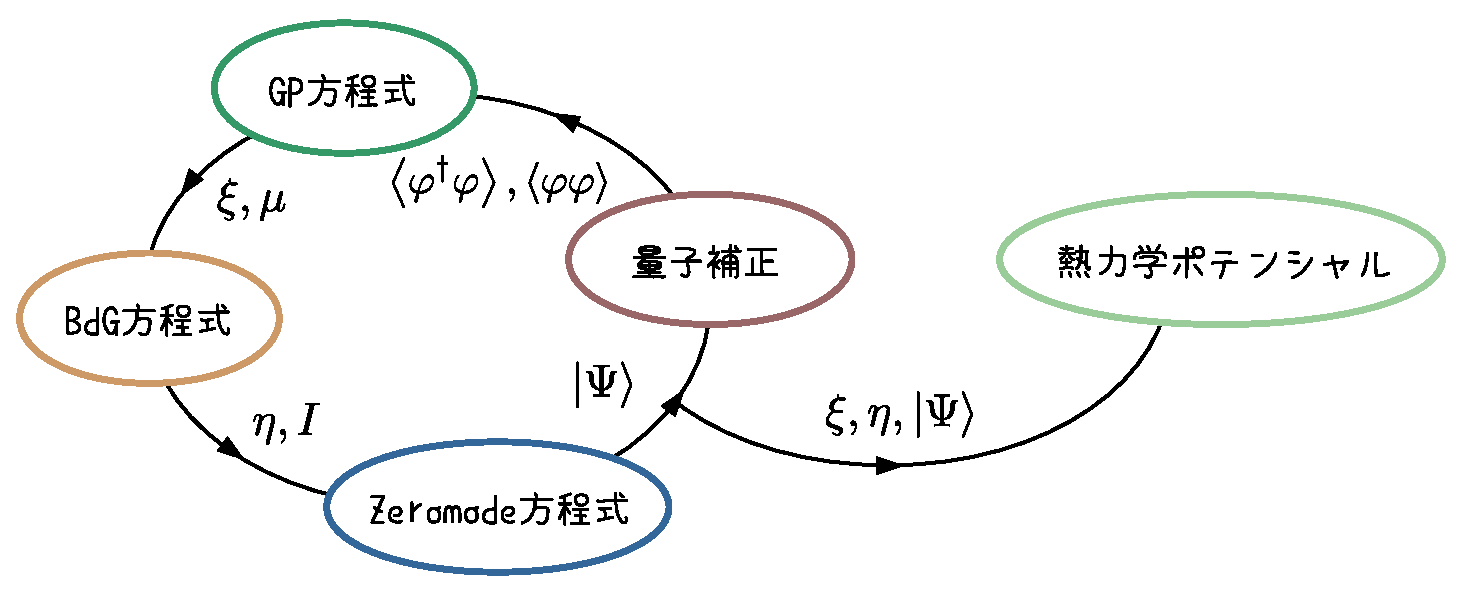
\includegraphics[width = 14cm]{./EPS/self-consistent_new2.eps}
\end{center}
\label{self-consistent}
\end{figure}

左の自己無撞着方程式が収束すると$\xi, \eta, \ket{\Psi}$が決まり, それによって分
配関数$Z$や, 熱力学ポテンシャル$\Omega$を(摂動的に)求めることが可能になる.
$\Omega$の摂動展開によって得られた熱力学関数はZeromode-BdG間の相互作用を一部取り
入れたものになっている.
\newpage
\section{一様系のFormulation}
\subsection{場の展開}
\begin{eqnarray}
  \varphi_{\rm ex} = \frac{1}{\sqrt{(2\pi)^3}}\int d\bm{k} \left[ u_ka_{\bm{k}} + v_k^*a^\dagger_{-\bm{k}} \right]e^{i\bm{k}\bm{x}}
\end{eqnarray}
\subsection{各演算子の期待値}
\begin{eqnarray}
  \ev{Q^2(s)}_z &=& \frac{\sum_mq^2\Psi_m(q)e^{-\beta E_m}}{\sum_me^{-\beta E_m}}\\
  \ev{P^2(s)}_z &=& \frac{-\sum_m\frac{d^2}{dq^2}\Psi_m(q)e^{-\beta E_m}}{\sum_me^{-\beta E_m}}\\
  \ev{a_{\bk}^\dagger(s) a_{\bk'}(s)}_{ex} &=& \frac{1}{e^{\beta\omega_{\bk}}-1}\delta(\bk-\bk') \equiv n_{\bk}\delta(\bk - \bk')\\
\nonumber  \ev{a_{\bk_1}^\dagger(s)a_{\bk_2}^\dagger(s) a_{\bk_3}(s)a_{\bk_4}(s)}_{ex} &=& \qty(\wick{12}{<1a^\dagger_{k1}<2a^\dagger_{k2}>1a_{k3}>2a_{k4}} + \wick{12}{<1a^\dagger_{k1}<2a^\dagger_{k2}>2a_{k3}>1a_{k4}})\\
  &=& n_{\bk_1}n_{\bk_2}\qty{\delta(\bk_1 - \bk_3)\delta(\bk_2 - \bk_4) + \delta(\bk_1 - \bk_4)\delta(\bk_2 - \bk_3)}
\end{eqnarray}
\subsection{量子補正項}
\begin{eqnarray}
  \ev{\varphi_{ex}\varphi_{ex}}_{ex} &=& \frac{1}{(2\pi)^3}\int d\bk_1\int d\bk_2 \ev{(u_{\bk_1}a_{\bk_1} + v_{\bk_1}^* a^\dagger_{-\bk_1})(u_{\bk_2}a_{\bk_2} + v_{\bk_2}^* a^\dagger_{-\bk_2})}_{ex}e^{i(\bk_1+\bk_2)\cdot \bx}\\
  &=& \frac{1}{(2\pi)^3}\int d\bk_1\int d\bk_2 \ev{(u_{\bk_1}a_{\bk_1} + v_{\bk_1}^* a^\dagger_{-\bk_1})(u_{\bk_2}a_{\bk_2} + v_{\bk_2}^* a^\dagger_{-\bk_2})}_{ex}e^{i(\bk_1+\bk_2)\cdot \bx}\\
  \nonumber &=& \frac{1}{(2\pi)^3}\int d\bk_1\int d\bk_2 \qty(u_{\bk_1}v_{\bk_2}^*\ev{a_{\bk_1} a^\dagger_{-\bk_2}}_{ex}\delta(\bk_1 + \bk_2) + v_{\bk_1}^* u_{\bk_2} \ev{a^\dagger_{-\bk_1}a_{\bk_2}}_{ex}\delta(\bk_1 + \bk_2))e^{i(\bk_1+\bk_2)\cdot \bx}\\
  \\
  &=& \frac{1}{(2\pi)^3}\int d\bk_1\int d\bk_2 \qty(u_{\bk_1}v_{-\bk_1}^*\ev{a_{\bk_1} a^\dagger_{\bk_1}}_{ex}\delta(\bk_1 + \bk_2) + v_{\bk_1}^* u_{-\bk_1} \ev{a^\dagger_{-\bk_1}a_{-\bk_1}}_{ex})\\
  &=& \frac{1}{(2\pi)^3}\int d\bk_1 \qty(u_{\bk_1}v_{-\bk_1}^*\ev{a_{\bk_1} a^\dagger_{\bk_1}}_{ex} + v_{\bk_1}^* u_{-\bk_1} \ev{a^\dagger_{-\bk_1}a_{-\bk_1}}_{ex})\\
  &=& \frac{1}{(2\pi)^3}\int d\bk_1 \qty(1+2n_{\bk})u_{\bk_1}v_{\bk_1} = \frac{1}{(2\pi)^3}\int_{+0}^\infty dk\ k^2\int_0^\pi d\theta\ \sin{\theta}\int_0^{2\pi} d\phi \qty(1+2n_k)u_kv_k\\
  &=& -\frac{1}{(2\pi)^2}\int_{+0}^\infty dk\frac{k^2\calM}{\omega_k}\qty(2n_k + 1)
\end{eqnarray}
となる. $\bk$積分について$\bk = 0$は含まれていないことに注意. この計算では
\begin{itemize}
\item[1. ]$u_{\pm\bk} = u_k, v_{\pm\bk} = v_k, n_{\pm\bk} = n_k$であること
\item[2. ]$\xi, \eta$が実であることで$v_k^* = v_k, u_k^* = u_k$
\item[3. ]$\ev{a_{\bk}a_{\bk}^\dagger}_{ex} = \ev{a_{\bk}^\dagger a_{\bk} + [a_{\bk}, a_{\bk}^\dagger]}_{ex} = 1 + n_k$であること
\item[4. ]$\int_{-\infty}^{\infty} d\bk\ev{a^\dagger_{-\bk}a_{-\bk}}_{ex} = \int_{-\infty}^{\infty} d\bk\ev{a^\dagger_{\bk}a_{\bk}}_{ex} = \int_{-\infty}^{\infty} d\bk n_k$であること
\end{itemize}
などを用いている. 各パラメータは以下の通り:
%$u_k, v_k, n_k, \calL_k...$などは2015夏の学校の資料を参照のこと. 同様にして
\begin{eqnarray}
  \begin{pmatrix}
      u_k\\
      v_k
    \end{pmatrix}
  &=& \frac{1}{\sqrt{2\omega_k}}
  \begin{pmatrix}
    \sqrt{{\cal L}_k + \omega_k}\\
    -\sqrt{{\cal L}_k - \omega_k}
  \end{pmatrix}\\
    {\cal M} = g(\xi^2 - \ev{\varphi\varphi})\hspace{1cm}{\cal L}_k &=& \frac{\hbar^2}{2m}k^2 + {\cal M}\hspace{1cm}\omega_k = \sqrt{\varepsilon_k(\varepsilon_k + 2gn_0)}= \sqrt{{\cal L}^2_k - {\cal M}^2}
\end{eqnarray}
同様にして, 
\begin{eqnarray}
  \ev{\varphi_{ex}^\dagger\varphi_{ex}}_{ex} &=& \frac{1}{(2\pi)^2}\int_0^\infty dk\frac{k^2}{\omega_k}\qty[(2n_k + 1)\calL_k - \omega_k]\\
  \ev{\varphi_{ex}^\dagger\varphi^\dagger_{ex}}_{ex} &=& -\frac{1}{(2\pi)^2}\int_0^\infty dk\frac{k^2\calM}{\omega_k}\qty(2n_k + 1)
\end{eqnarray}
相互作用項は
\begin{eqnarray}
\nonumber  \ev{\varphi_{ex}^\dagger\varphi_{ex}^\dagger\varphi_{ex}\varphi_{ex}}_{ex} &=& \frac{1}{(2\pi)^6}\int d\bk_1\int d\bk_2\int d\bk_3\int d\bk_4 e^{i(-\bk_1-\bk_2+\bk_3+\bk_4)\cdot \bx}\\
\nonumber  &\times& \ev{(u_{\bk_1} a_{\bk_1}^\dagger + v_{\bk_1}a_{-\bk_1})(u_{\bk_2} a_{\bk_2}^\dagger + v_{\bk_2}a_{-\bk_2})(u_{\bk_3} a_{\bk_3} + v_{\bk_3}a_{-\bk_3}^\dagger)(u_{\bk_4} a_{\bk_4} + v_{\bk_4}a_{-\bk_4}^\dagger)}_{ex}\\
\end{eqnarray}
である. 生成演算子と消滅演算子が対になっていない期待値は消えてしまうので, 残るものだけを書き下す:
\begin{eqnarray}
  \nonumber  \ev{\varphi_{ex}^\dagger\varphi_{ex}^\dagger\varphi_{ex}\varphi_{ex}}_{ex} &=& \frac{1}{(2\pi)^6}\int d\bk_1\int d\bk_2\int d\bk_3\int d\bk_4 e^{i(-\bk_1-\bk_2+\bk_3+\bk_4)\cdot \bx}\\
  \nonumber  &\times& \Bigl[u_{\bk_1}u_{\bk_2}u_{\bk_3}u_{\bk_4}\ev{a^\dagger_{\bk_1}a^\dagger_{\bk_2}a_{\bk_3}a_{\bk_4}}_{ex} + u_{\bk_1}v_{\bk_2}u_{\bk_3}v_{\bk_4}\ev{a^\dagger_{\bk_1}a_{-\bk_2}a_{\bk_3}a^\dagger_{-\bk_4}}_{ex}\\
    \nonumber    &&+ u_{\bk_1}v_{\bk_2}v_{\bk_3}u_{\bk_4}\ev{a^\dagger_{\bk_1}a_{-\bk_2}a^\dagger_{-\bk_3}a_{\bk_4}}_{ex} + v_{\bk_1}u_{\bk_2}u_{\bk_3}v_{\bk_4}\ev{a_{-\bk_1}a^\dagger_{\bk_2}a_{\bk_3}a^\dagger_{-\bk_4}}_{ex}\\
\nonumber    &&+ v_{\bk_1}u_{\bk_2}v_{\bk_3}u_{\bk_4}\ev{a_{-\bk_1}a^\dagger_{\bk_2}a^\dagger_{-\bk_3}a_{\bk_4}}_{ex} + v_{\bk_1}v_{\bk_2}v_{\bk_3}v_{\bk_4}\ev{a_{-\bk_1}a_{-\bk_2}a^\dagger_{-\bk_3}a^\dagger_{-\bk_4}}_{ex}\Bigr]\\\label{interaction-expectation}
\end{eqnarray}
Wickの定理で展開:
\begin{eqnarray}
\nonumber  \ev{a^\dagger_{\bk_1}a^\dagger_{\bk_2}a_{\bk_3}a_{\bk_4}}_{ex} &=& \qty(\wick{12}{<1a^\dagger_{k1}<2a^\dagger_{k2}>1a_{k3}>2a_{k4}} + \wick{21}{<1a^\dagger_{k1}<2a^\dagger_{k2}>2a_{k3}>1a_{k4}})\\
&=& n_{\bk_1}n_{\bk_2}\qty{\delta(\bk_1 - \bk_3)\delta(\bk_2 - \bk_4) + \delta(\bk_1 - \bk_4)\delta(\bk_2 - \bk_3)}\\
\nonumber  \ev{a^\dagger_{\bk_1}a_{-\bk_2}a_{\bk_3}a^\dagger_{-\bk_4}}_{ex} &=& \qty(\wick{12}{<1a^\dagger_{k1}>1a_{-k2}<2a_{k3}>2a^\dagger_{-k4}} + \wick{12}{<1a^\dagger_{k1}<2a_{-k2}>1a_{k3}>2a^\dagger_{-k4}})\\
\nonumber&=& n_{\bk_1}(1 + n_{\bk_3})\delta(\bk_1 + \bk_2)\delta(\bk_3 + \bk_4) + n_{\bk_1}(1 + n_{\bk_2})\delta(\bk_1 - \bk_3)\delta(\bk_2 - \bk_4)\\
\\
\nonumber  \ev{a^\dagger_{\bk_1}a_{-\bk_2}a^\dagger_{-\bk_3}a_{\bk_4}}_{ex} &=& \qty(\wick{12}{ <1a^\dagger_{k_1}>1a_{-k_2}<2a^\dagger_{-k_3}>2a_{k_4}} + \wick{21}{<1a^\dagger_{k_1}<2a_{-k_2}>2a^\dagger_{-k_3}>1a_{k_4}})\\
&=& n_{\bk_1}n_{\bk_3}\delta(\bk_1 + \bk_2)\delta(\bk_3 + \bk_4) + n_{\bk_1}(1 + n_{\bk_2})\delta(\bk_1 - \bk_4)\delta(\bk_2 - \bk_3)\\
\nonumber  \ev{a_{-\bk_1}a^\dagger_{\bk_2}a_{\bk_3}a^\dagger_{-\bk_4}}_{ex} &=& \qty(\wick{12}{<1a_{-k_1}>1a^\dagger_{k_2}<2a_{k_3}>2a^\dagger_{-k_4}} + \wick{21}{<1a_{-k_1}<2a^\dagger_{k_2}>2a_{k_3}>1a^\dagger_{-k_4}})\\
\nonumber&=& (1+n_{\bk_1})(1+n_{\bk_3})\delta(\bk_1 + \bk_2)\delta(\bk_3 + \bk_4) + (1+n_{\bk_1})n_{\bk_2}\delta(\bk_1 - \bk_4)\delta(\bk_2 - \bk_3)\\
\\
\nonumber  \ev{a_{-\bk_1}a^\dagger_{\bk_2}a^\dagger_{-\bk_3}a_{\bk_4}}_{ex} &=& \qty(\wick{12}{<1a_{-k_1}>1a^\dagger_{k_2}<2a^\dagger_{-k_3}>2a_{k_4}} + \wick{12}{<1a_{-k_1}<2a^\dagger_{k_2}>1a^\dagger_{-k_3}>2a_{k_4}})\\
&=& (1 + n_{\bk_1})n_{\bk_3}\delta(\bk_1 + \bk_2)\delta(\bk_3 + \bk_4) + (1 + n_{\bk_1})n_{\bk_2}\delta(\bk_1 - \bk_3)\delta(\bk_2 - \bk_4)\\
\nonumber  \ev{a_{-\bk_1}a_{-\bk_2}a^\dagger_{-\bk_3}a^\dagger_{-\bk_4}}_{ex} &=& \qty(\wick{12}{<1a_{-k_1}<2a_{-k_2}>1a^\dagger_{-k_3}>2a^\dagger_{-k_4}} + \wick{21}{<1a_{-k_1}<2a_{-k_2}>2a^\dagger_{-k_3}>1a^\dagger_{-k_4}})\\
&=& (1 + n_{\bk_1})(1 + n_{\bk_2})\qty{\delta(\bk_1 - \bk_3)\delta(\bk_2 - \bk_4) + \delta(\bk_1 - \bk_4)\delta(\bk_2 - \bk_3)}
\end{eqnarray}
これらを(\ref{interaction-expectation})に代入すると
\begin{eqnarray}
  \ev{\varphi_{ex}^\dagger\varphi_{ex}^\dagger\varphi_{ex}\varphi_{ex}}_{ex} &=& \frac{1}{(2\pi)^6}\qty[2\qty(I_u'^{, 2} + I_v'^{+, 2} +  I_u'I_v'^{+} + I_{uv}I_{uv}^+) + I_{uv}^2 + I_u'I_v'^+ + I_{uv}^{+, 2} + I_u'^{+}I_v']\\
  &=& \frac{1}{(2\pi)^6}\qty[2\qty(I_u'^{, 2} + I_v'^{+, 2} +  I_u'I_v'^{+}) + \qty(I_{uv} + I_{uv}^{+})^2+ I_u'I_v'^+  + I_u'^{+}I_v']\\
  &=& \frac{1}{(2\pi)^6}\qty[2\qty(I_u'^{, 2} + I_v'^{+, 2}) + \qty(I_{uv} + I_{uv}^{+})^2+ 4I_u'I_v'^+]
\end{eqnarray}
となる. ただし
\begin{eqnarray}
\nonumber I_u' &=& \int d\bk n_{\bk} u_{\bk}^2\hspace{1cm}I_v' = \int d\bk n_{\bk} v_{\bk}^2\hspace{1cm} I_{uv} = \int d\bk n_{\bk} u_{\bk}v_{\bk}\\
\nonumber I_{uv}^+ &=& \int d\bk (1 + n_{\bk}) u_{\bk}v_{\bk} \hspace{1cm}I_v'^+ = \int d\bk (1 + n_{\bk}) v_{\bk}^2\hspace{1cm}I_u'^+ = \int d\bk (1 + n_{\bk}) u_{\bk}^2\\
\end{eqnarray}
であり, かつ$I_u'I_v'^+ = I_u'^+I_v'$であることを用いている.

以上で具体的にゼロモード・励起モードの期待値が計算できたので,
(\ref{Hamiltonian-Exp})に(\ref{Zeromode-Exp}), (\ref{BdG-Exp}),
(\ref{Interaction-Exp})を代入する.$I$はすべて$\bx$依存性を持たないので空間積分は系の体積$V$が出てくるだけ.
まとめると, (\ref{Hamiltonian-Exp})は
\begin{eqnarray}
  \nonumber  \ev{H_{\rm int}}_0 =&& \int d\bx\Bigl[-\frac{2}{(2\pi)^2}\qty(-\xi^2\ev{Q^2}_z + \eta^2\ev{P^2}_z)\int_{+0}^\infty dk\frac{k^2\calM}{\omega_k}\qty(2n_k + 1)\\
    &+& \frac{4}{(2\pi)^2}\qty(\xi^2\ev{Q^2}_z + \eta^2\ev{P^2}_z)\int_0^\infty dk\frac{k^2}{\omega_k}\qty{(2n_k + 1)\calL_k - \omega_k}\\
    &+& \frac{1}{(2\pi)^6}\qty{2\qty(I_u'^{, 2} + I_v'^{+, 2}) + \qty(I_{uv} + I_{uv}^{+})^2+ 4I_u'I_v'^+}\Bigr]
\end{eqnarray}

